% The Slide Definitions
%document
\documentclass[10pt]{beamer}
%theme
\usetheme{metropolis}
% packages
\usepackage{color}
\usepackage{listings}
\usepackage[ngerman]{babel}
\usepackage[utf8]{inputenc}
\usepackage{multicol}


% color definitions
\definecolor{mygreen}{rgb}{0,0.6,0}
\definecolor{mygray}{rgb}{0.5,0.5,0.5}
\definecolor{mymauve}{rgb}{0.58,0,0.82}

\lstset{
    backgroundcolor=\color{white},
    % choose the background color;
    % you must add \usepackage{color} or \usepackage{xcolor}
    basicstyle=\footnotesize\ttfamily,
    % the size of the fonts that are used for the code
    breakatwhitespace=false,
    % sets if automatic breaks should only happen at whitespace
    breaklines=true,                 % sets automatic line breaking
    captionpos=b,                    % sets the caption-position to bottom
    commentstyle=\color{mygreen},    % comment style
    % deletekeywords={...},
    % if you want to delete keywords from the given language
    extendedchars=true,
    % lets you use non-ASCII characters;
    % for 8-bits encodings only, does not work with UTF-8
    frame=single,                    % adds a frame around the code
    keepspaces=true,
    % keeps spaces in text,
    % useful for keeping indentation of code
    % (possibly needs columns=flexible)
    keywordstyle=\color{blue},       % keyword style
    % morekeywords={*,...},
    % if you want to add more keywords to the set
    numbers=left,
    % where to put the line-numbers; possible values are (none, left, right)
    numbersep=5pt,
    % how far the line-numbers are from the code
    numberstyle=\tiny\color{mygray},
    % the style that is used for the line-numbers
    rulecolor=\color{black},
    % if not set, the frame-color may be changed on line-breaks
    % within not-black text (e.g. comments (green here))
    stepnumber=1,
    % the step between two line-numbers.
    % If it's 1, each line will be numbered
    stringstyle=\color{mymauve},     % string literal style
    tabsize=4,                       % sets default tabsize to 4 spaces
    % show the filename of files included with \lstinputlisting;
    % also try caption instead of title
    language = Python,
	showspaces = false,
	showtabs = false,
	showstringspaces = false,
	escapechar = ,
}

\def\ContinueLineNumber{\lstset{firstnumber=last}}
\def\StartLineAt#1{\lstset{firstnumber=#1}}
\let\numberLineAt\StartLineAt



\newcommand{\codeline}[1]{
	\alert{\texttt{#1}}
}


% Author and Course information
% This Document contains the information about this course.

% Authors of the slides
\author{Philipp Hanisch, Valentin Roland}

% Name of the Course
\institute{Python-Grundlagen}

% Fancy Logo 
\titlegraphic{\hfill
\includegraphics[height=1.25cm]{fsr_logo_cropped}}



% Custom Bindings
% \newcommand{\codeline}[1]{
%	\alert{\texttt{#1}}
%}


% Presentation title
\title{Verwenden von Bibliotheken: Matplotlib}
\date{\today}


\begin{document}

\maketitle

\section{Rückblick}

\begin{frame}{Aufgaben}
	\begin{enumerate}
		\item Erweitere die Spielerklasse, sodass ein Spieler mehrere Würfel besitzen kann. Wenn er würfelt, so soll er mit allen Würfeln nacheinander würfeln und eine Ergebnisliste zurückbekommen.
		\item Modelliert das Würfelspiel als eigene Klasse.
	\end{enumerate}
    $\hookrightarrow$ Lösung in Snippets
\end{frame}

\begin{frame}[fragile]{Module einbinden}
	\begin{lstlisting}
from random import randint
print(randint(1, 10))

from wuerfel import *
d20 = Wuerfel(20)
print(d20.wuerfeln())

import spieler
spieler = spieler.Spieler("Arndt", d20)
print(spieler.name)
	\end{lstlisting}
\end{frame}

\section{matplotlib}

\begin{frame}{Motivation}
    \begin{itemize}
        \item Mit Python berechnete Daten plotten:
        \begin{figure}[h]
            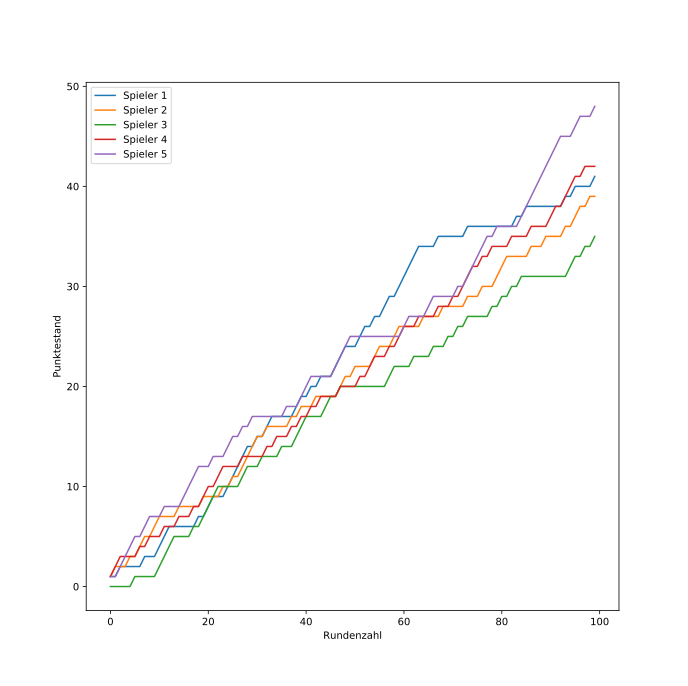
\includegraphics[width = .7\linewidth]{spielplot}
        \end{figure}
    \end{itemize}
\end{frame}

\begin{frame}[fragile]{Einfaches Beispiel}
    \begin{lstlisting}
from matplotlib import pyplot
pyplot.plot([1,2,3,4], [1,4,9,16], 'ro')
pyplot.axis([0, 6, 0, 20])
pyplot.show()
    \end{lstlisting}

    \begin{figure}[h]
        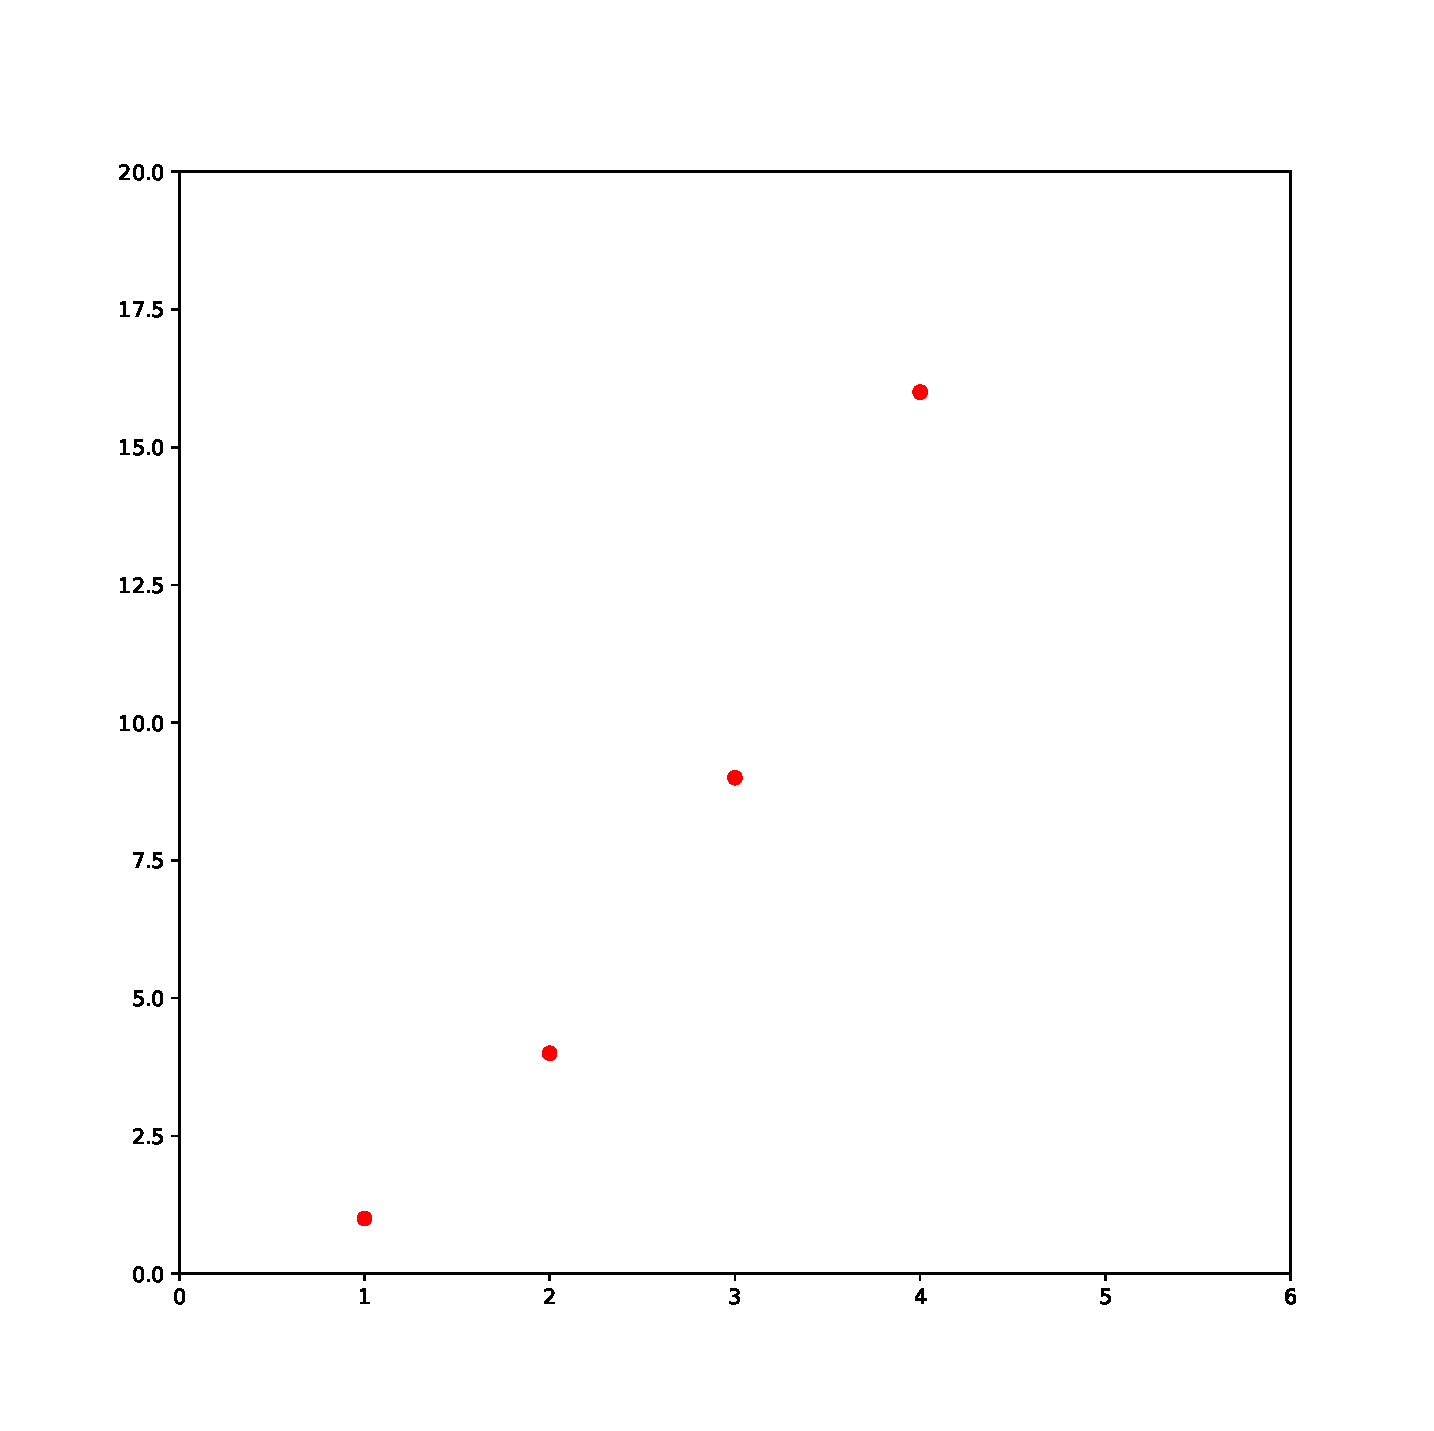
\includegraphics[width=.5\linewidth]{matplotlib_example1}
    \end{figure}
\end{frame}

\begin{frame}[fragile]{Matplotlib instalieren}
    Linux (Ubuntu):
    \begin{lstlisting}
        pip3 install --user matplotlib
    \end{lstlisting}

    Windows:
    \begin{lstlisting}
        python.exe -m pip install matplotlib
    \end{lstlisting}
    Matplotlib Tutorial: \url{https://matplotlib.org/users/pyplot_tutorial.html}
\end{frame}

\section{Aufgaben}

\begin{frame}{Aufgaben}
    \begin{enumerate}
        \item Erstelle ein Diagramm, in dem der Entstand eines Spiels nach der Simulation (\texttt{.simuliere()}) für jeden Spieler dargestellt ist.
        \item Erstelle ein Diagramm, in dem der Punktestand aller Spieler im zeitlichen Verlauf dargestellt ist (s. Beispiel in dieser Präsentation)
        \item Füge einen schummelnden Spieler zu deinem Spiel hinzu:
            \begin{enumerate}
                \item Mehr Würfel
                \item Andere Seitenzahl
                \item seid kreativ $\dots$
            \end{enumerate}
            Wie wirkt sich das Schummeln bei den verschiedenen Wertungsmodi aus? \\
            (\texttt{"wuerfelsumme"}, \texttt{"wuerfelmaximum"}, \texttt{"paschzahl"})\\
            Dies wird bei höherer Rundenzahl möglicherweise deutlicher.
    \end{enumerate}
\end{frame}



\end{document}
